\documentclass[11pt]{article}
\usepackage{algorithm2e}
\usepackage[italian]{babel}
\usepackage[document]{ragged2e}
\usepackage{amsfonts, amssymb, amsmath}
\usepackage{cancel}
\usepackage{float}
\usepackage{mathtools}
\usepackage[margin=3cm]{geometry}
\usepackage{subfig}
\usepackage{mwe}
\usepackage{hyperref}

\tolerance=1
\emergencystretch=\maxdimen
\hyphenpenalty=10000
\hbadness=10000

\begin{document}
\graphicspath{ {./img/} }
\begin{titlepage}
    \begin{center}
        \vspace*{1.5cm}
            
        \Huge
        \textbf{IMAGING}
            
        \vspace{0.5cm}
        \LARGE
        Relazione
            
        \vspace{1.5cm}
          
        \begin{minipage}[t]{0.47\textwidth}
        \begin{center}
        	{\large{\bf Cheikh Ibrahim $\cdot$ Zaid}}\\
			{\large Matricola: \texttt{0000974909}}
        \end{center}

		\end{minipage}
		\hfill
		\begin{minipage}[t]{0.47\textwidth}\raggedleft
		\begin{center}
        	{\large{\bf Xia $\cdot$ Tian Cheng}}\\
			{\large Matricola: \texttt{0000975129}}
        \end{center}
		\end{minipage}  
            
        \vspace{6cm}
            
        Anno accademico\\
        $2021 - 2022$
            
        \vspace{0.8cm}
            
            
        \Large
        Corso di Calcolo Numerico\\
        Alma Mater Studiorum $\cdot$ Università di Bologna\\
            
    \end{center}
\end{titlepage}
\pagebreak

\section{Introduzione}
Il progetto consiste nel ricostruire un'immagine a partire da una sua istanza alterata da uno sfocamento noto e un rumore casuale.\\
Si tratta di un problema solitamente affrontato elaborando immagini provenienti da un dispositivo di acquisizione che nel suo processo di cattura deve digitalizzare un segnale analogico. 
Per risolvere tali problemi sono note diverse formulazioni. Quelle impiegate per questo progetto sono:
\begin{itemize}
    \setlength\itemsep{0.05cm}
    \item Minimi quadrati
    \item Minimi quadrati con regolarizzazione di Tikhonov
    \item Minimi quadrati con regolarizzazione tramite variazione totale
\end{itemize}
È noto che risolvere il problema di deblur come minimi quadrati in modo diretto è mal condizionato e per questo si introducono tecniche di regolarizzazione.\\
Per misurare la qualità dei risultati verranno impiegate due metriche:
\begin{itemize}
    \setlength\itemsep{0.05cm}
    \item Mean Squared Error (MSE) \textbf{[AGGIUNGERE DESCRIZIONE]}
    \item Peak Signal-to-Noise Ratio (PSNR) \textbf{[AGGIUNGERE DESCRIZIONE]}
\end{itemize}

\section{Esecuzione preliminare}
Per avere una visione sul comportamento delle varie formulazioni, è stata eseguita una prima sperimentazione sull'immagine in \autoref{fig:originale1}
\begin{figure}[H]
    \centering
    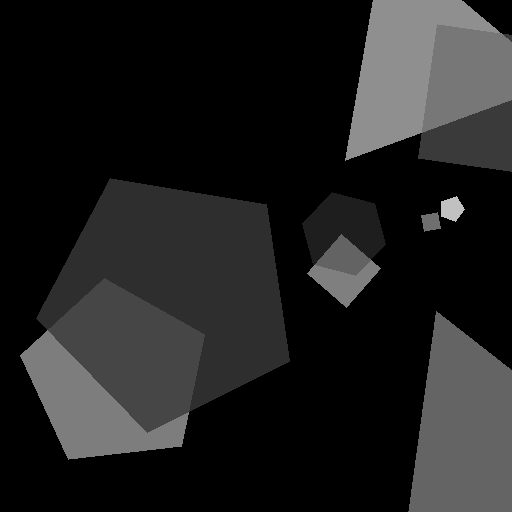
\includegraphics[width=4cm]{esecuzione/originale.png}
    \caption{Immagine di test}
    \label{fig:originale1}
\end{figure}

\subsection{Prima esecuzione}
La prima esecuzione è stata eseguita con un kernel $5 \times 5$ con $\sigma=0.5$ e rumore gaussiano con deviazione standard $]0, 0.05]$.

\subsubsection{Stima di $\lambda$}
Per valutare il risultato dei vari metodi, è necessario prima determinare il valore $\lambda$ del termine di regolarizzazione degli algoritmi che lo prevedono.
Il seguente grafico mostra il valore del PSNR al variare di $\lambda \in [0.01, 1]$ con passo $0.01$:
\begin{figure}[H]
    \centering
    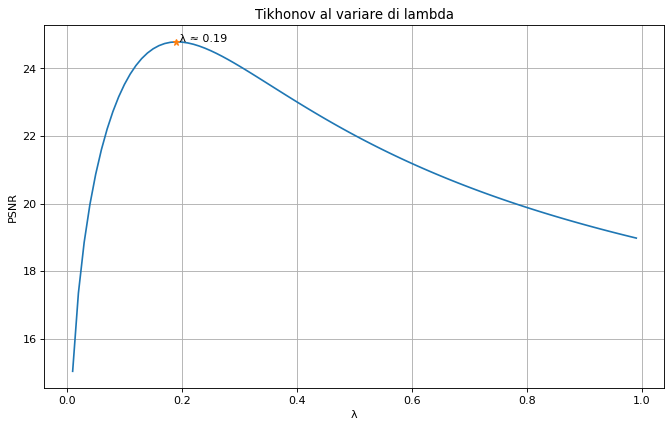
\includegraphics[width=10cm]{esecuzione/1/tikhonov_lambda.png}
    \caption{$\lambda=0.19$ e $\texttt{PSNR} \simeq 24.79$}
    \label{fig:tikhonov_lambda1}
\end{figure}
Analogamente, il seguente grafico mostra la variazione del PSNR per $\lambda \in [0.01, 1]$ con passo $0.01$:
\begin{figure}[H]
    \centering
    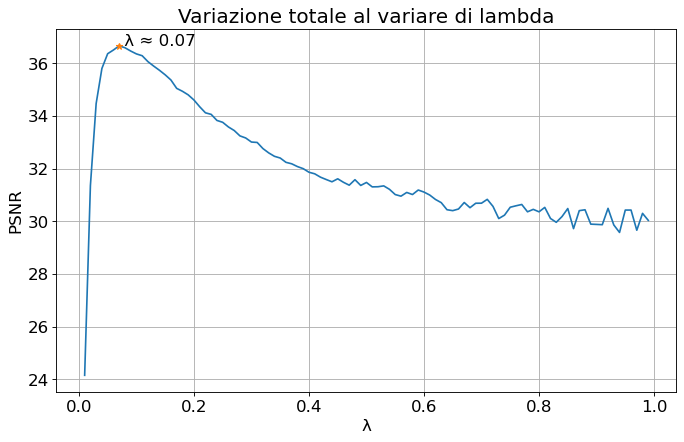
\includegraphics[width=10cm]{esecuzione/1/tv_lambda.png}
    \caption{$\lambda=0.07$ e $\texttt{PSNR} \simeq 36.74$}
    \label{fig:tv_lambda1}
\end{figure}

\subsubsection{Esecuzione}
I risultati della prima esecuzione sono osservabili in \autoref{fig:deblur1}.\\
\begin{figure}[H]
    \centering
    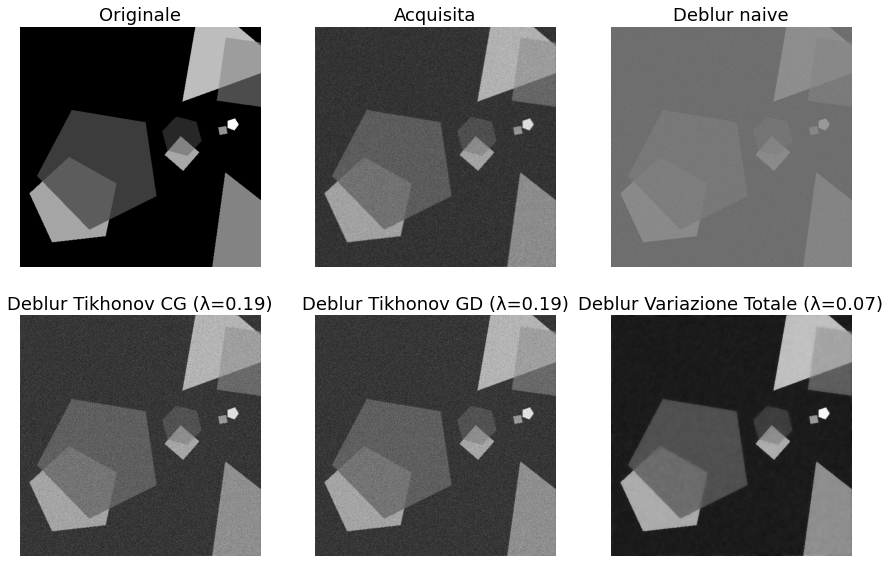
\includegraphics[width=13cm]{esecuzione/1/deblur.png}
    \caption{Risultato sulle varie formulazioni}
    \label{fig:deblur1}
\end{figure}

\begin{center}
    \begin{tabular}{ |c|c|c|c|c|c| }
    \hline
    & Acquisita & Naive & Tikhonov CG & Tikhonov GD & Variazione totale \\ 
    \hline
    MSE & $0.2699 \cdot 10^{-2}$ & $0.2047 \cdot 10^{0}$ & $0.33197 \cdot 10^{-2}$ & $0.3320 \cdot 10^{-2}$ & $0.2119 \cdot 10^{-3}$ \\ 
    PSNR & $25.6878$ & $6.8874$ & $24.7890$ & $24.7890$ & $36.7382$ \\ 
    Iter. & & 140 & 14 & 48 & 14 \\ 
    \hline
    \end{tabular}
\end{center}

Come atteso, il risultato ottenuto con la formulazione come problema ai minimi quadrati senza regolarizzazione ha prodotto un'immagine molto distante dall'originale.\\
Utilizzando la regolarizzazione di Tikhonov, si è ottenuto un risultato quasi invariato rispetto all'immagine acquisita se non addirittura peggiore; mentre a livello di velocità, il metodo del gradiente ha richiesto più iterazioni rispetto al metodo del gradiente coniugato.\\
Con la regolarizzazione tramite variazione totale, il risultato ottenuto è invece migliore rispetto agli altri metodi e molto vicina all'immagine originale.\\
La ragione per cui Tikhonov ha prodotto tale risultato è probabilmente dovuto al fatto che il rumore "sovrasta" il blur.

\subsection{Seconda esecuzione}
Per vedere le prestazioni di Tikhonov in uno scenario differente, è stata effettuata una seconda esecuzione sulla stessa immagine di partenza con blur ottenuto da un kernel $24 \times 24$ con $\sigma=3$ e rumore con deviazione standard $]0, 0.05]$.

\subsubsection{Stima di $\lambda$}
\begin{figure}[H]
    \centering
    \begin{minipage}{0.45\textwidth}
        \centering
        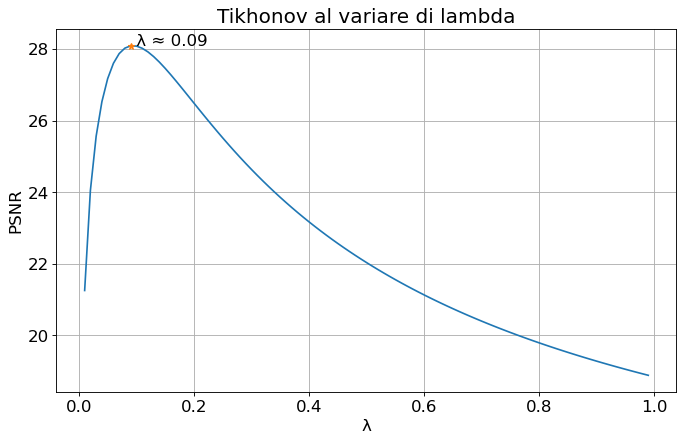
\includegraphics[width=7cm]{esecuzione/2/tikhonov_lambda.png}
        \caption{$\lambda=0.09$ e $\texttt{PSNR} \simeq 28.09$}
        \label{fig:tikhonov_lambda2}
    \end{minipage}\hfill
    \begin{minipage}{0.45\textwidth}
        \centering
        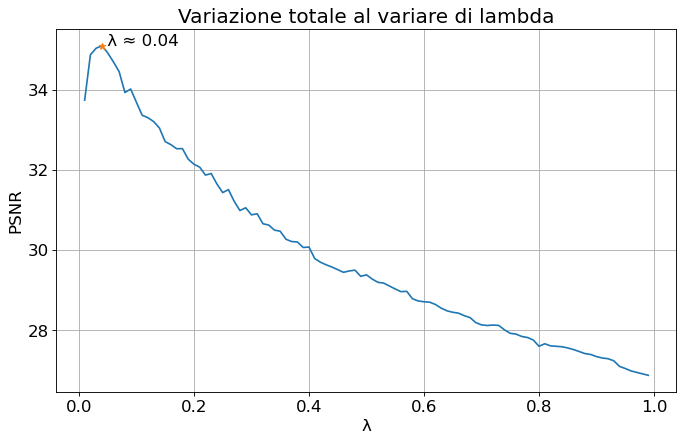
\includegraphics[width=7cm]{esecuzione/2/tv_lambda.png}
        \caption{$\lambda=0.04$ e $\texttt{PSNR} \simeq 35.09$}
        \label{fig:tv_lambda2}
    \end{minipage}
\end{figure}

\subsubsection{Esecuzione}
I risultati sono rappresentati in \autoref{fig:deblur2}.\\
\begin{figure}[H]
    \centering
    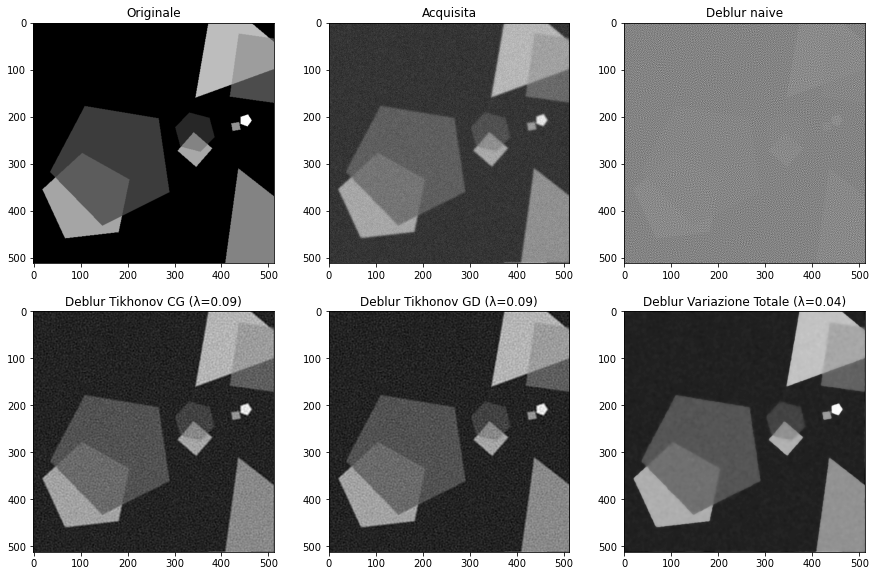
\includegraphics[width=13cm]{esecuzione/2/deblur.png}
    \caption{Risultato sulle varie formulazioni}
    \label{fig:deblur2}
\end{figure}

\begin{center}
    \begin{tabular}{ |c|c|c|c|c|c| }
    \hline
    & Acquisita & Naive & Tikhonov CG & Tikhonov GD & Variazione totale \\ 
    \hline
    MSE & $0.3204 \cdot 10^{-2}$ & $0.5719 \cdot 10^{-1}$ & $0.1553 \cdot 10^{-2}$ & $0.1553 \cdot 10^{-2}$ & $0.3094 \cdot 10^{-3}$ \\ 
    PSNR & $24.9437$ & $-7.5735$ & $28.0889$ & $28.0890$ & $35.0944$ \\ 
    Iter. & & 200 (max) & 18 & 99 & 29 \\ 
    \hline
    \end{tabular}
\end{center}

Anche in questo caso, il metodo naive non ha prodotto soluzioni accettabili, mentre la regolarizzazione tramite variazione totale, come nel caso precedente, ha prodotto il risultato migliore.\\
Il metodo regolarizzato con Tikhonov invece, a differenza dell'esecuzione precedente, ha prodotto un risultato migliore dell'immagine acquisita e, 
analogamente, il numero di iterazioni del metodo che minimizza con il gradiente coniugato è minore rispetto al metodo del gradiente.

\section{Confronto tra gradiente coniugato e metodo del gradiente}
\label{chap:confronto}
Si analizzano ora le prestazioni di Tikhonov utilizzando i due metodi di discesa implementati. \\

\subsection{Prima esecuzione}
Per una prima sperimentazione si è usata la \autoref{fig:originale1} con kernel $5 \times 5$ con $\sigma=0.5$ e rumore gaussiano con deviazione standard $]0, 0.05]$.\\
I risultati ottenuti sono i seguenti:
\begin{figure}[H]
    \centering
    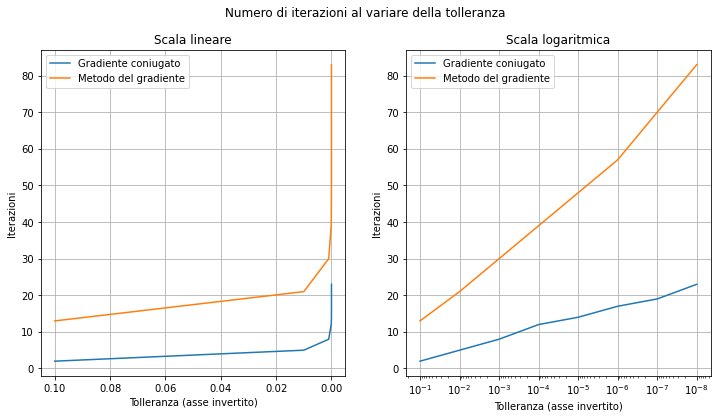
\includegraphics[width=10cm]{iterazioni_cg_gd/1/tol_iter.png}
    \caption{Iterazioni al variare della tolleranza}
    \label{fig:tol_iter1}
\end{figure}
È immediato notare che il metodo del gradiente coniugato impiega meno iterazioni rispetto al metodo del gradiente.\\

\begin{figure}[H]
    \centering
    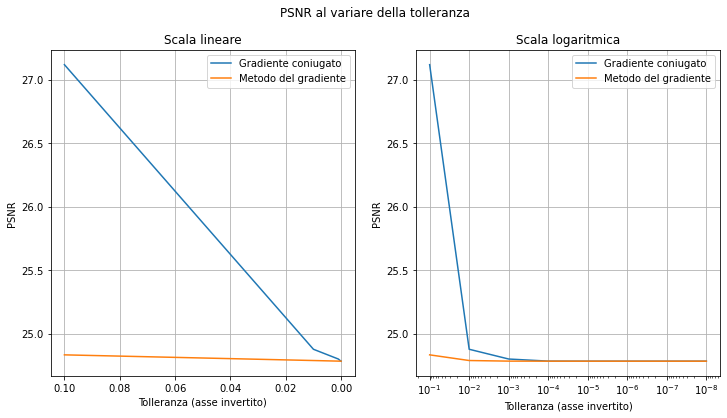
\includegraphics[width=10cm]{iterazioni_cg_gd/1/tol_psnr.png}
    \caption{PSNR al variare della tolleranza}
    \label{fig:tol_psnr1}
\end{figure}
Il risultato ottenuto mostra che i due metodi, al variare della tolleranza, convergono allo stesso risultato.\\
È però presente un comportamento controintuitivo in vicinanza di valori di tolleranza elevati. 
Infatti si ottiene un PSNR maggiore in corrispondenza di tali valori, in altri termini, si ottiene un'immagine più fedele all'originale con meno iterazioni, mentre il risultato peggiora nella continuazione dell'esecuzione (Tale problematica verrà approfondita nella \autoref{chap:semiconv}).

\begin{figure}[H]
    \centering
    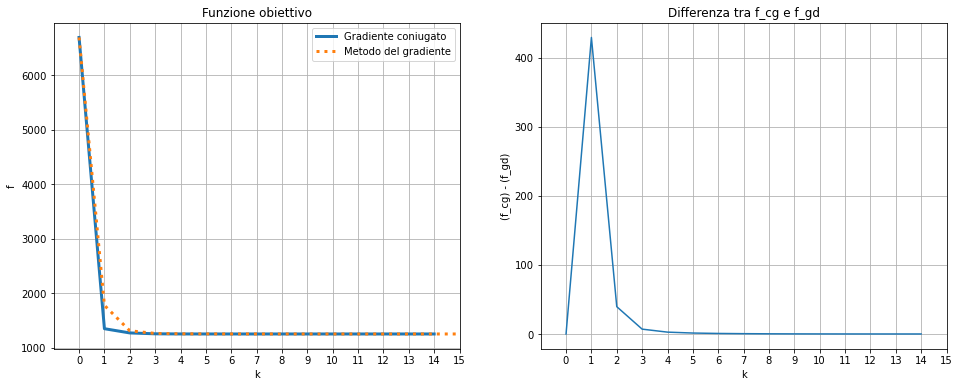
\includegraphics[width=10cm]{iterazioni_cg_gd/1/funzione_obiettivo.png}
    \caption{Andamento della funzione obiettivo}
    \label{fig:obiettivo1}
\end{figure}
\begin{figure}[H]
    \centering
    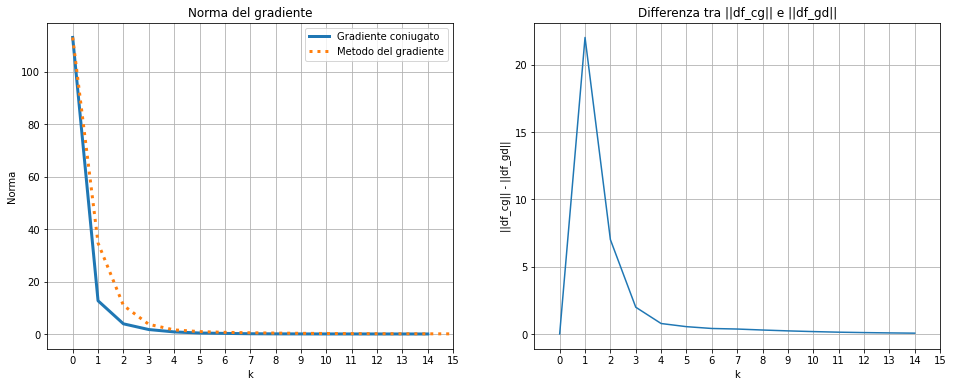
\includegraphics[width=10cm]{iterazioni_cg_gd/1/norma_gradiente.png}
    \caption{Andamento della norma del gradiente}
    \label{fig:gradiente1}
\end{figure}
Come atteso dai risultati precedenti, per il metodo del gradiente coniugato la decrescita della funzione obiettivo è maggiore rispetto al metodo del gradiente. 
Lo stesso risultato è osservabile con la norma del gradente che nel caso del gradiente coniugato esegue "salti" di dimensione maggiore.

\subsection{Seconda esecuzione}
Per una seconda valutazione si è usato un kernel $24 \times 24$ con $\sigma=3$ e rumore gaussiano con deviazione standard $]0, 0.05]$.\\

\begin{figure}[H]
    \centering
    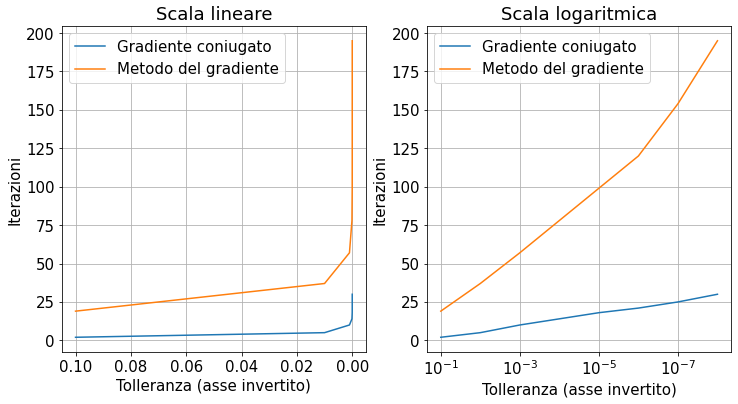
\includegraphics[width=10cm]{iterazioni_cg_gd/2/tol_iter.png}
    \caption{Iterazioni al variare della tolleranza}
    \label{fig:tol_iter2}
\end{figure}
\begin{figure}[H]
    \centering
    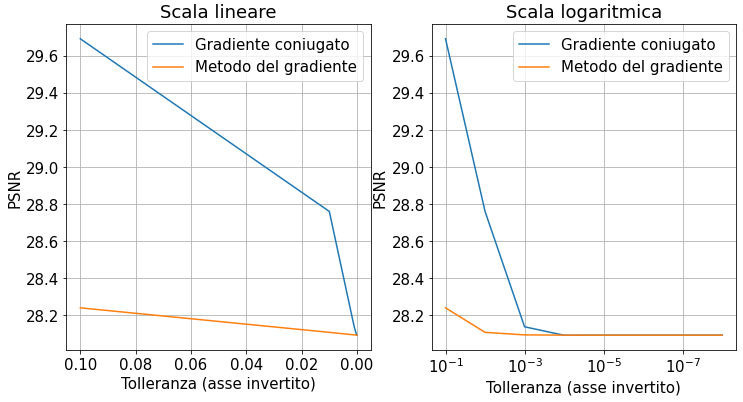
\includegraphics[width=10cm]{iterazioni_cg_gd/2/tol_psnr.png}
    \caption{PSNR al variare della tolleranza}
    \label{fig:tol_psnr2}
\end{figure}
\begin{figure}[H]
    \centering
    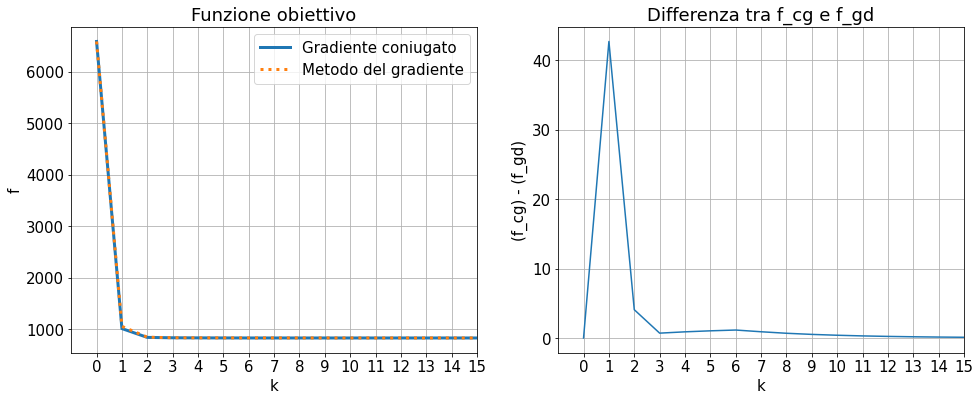
\includegraphics[width=10cm]{iterazioni_cg_gd/2/funzione_obiettivo.png}
    \caption{Andamento della funzione obiettivo}
    \label{fig:obiettivo2}
\end{figure}
\begin{figure}[H]
    \centering
    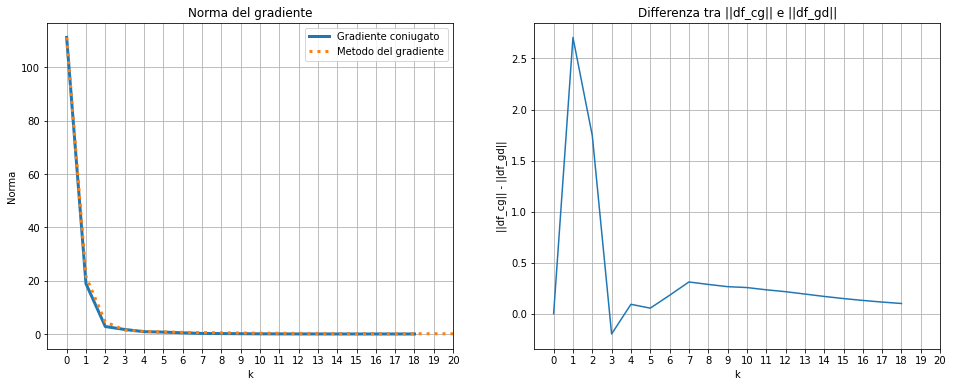
\includegraphics[width=10cm]{iterazioni_cg_gd/2/norma_gradiente.png}
    \caption{Andamento della norma del gradiente}
    \label{fig:gradiente2}
\end{figure}

I risultati ottenuto sono in linea con quelli precedenti ed evidenziano che le prestazioni del gradiente coniugato sono maggiori rispetto a quelle del metodo del gradiente, come atteso dalle valutazioni teoriche.

\section{Semi-convergenza}
\label{chap:semiconv}
Nella \autoref{chap:confronto} è emerso il problema per cui l'immagine ottenuta con meno iterazioni è migliore rispetto a quella ottenuta quando il metodo raggiunge convergenza. 
Tale problema è noto come semi-convergenza, ovvero metodi per il quale il raggiungimento dell'ottimo non corrisponde al soddisfacimento delle condizioni di convergenza 
e per questo le iterazioni successive peggiorano il risultato.\\
Nel contesto del deblur, il problema di semi-convergenza è causato dal rumore aggiunto all'immagine. È noto che il metodo naive è quello che più viene condizionato dal rumore e per questa ragione vengono introdotti i metodi di regolarizzazione.\\
Si analizza quindi il risultato dei vari metodi analizzando l'andamento dell'iterato $x_{k}$:

\subsection{Analisi con rumore}
\subsubsection{Metodo naive}
\begin{figure}[H]
    \centering
    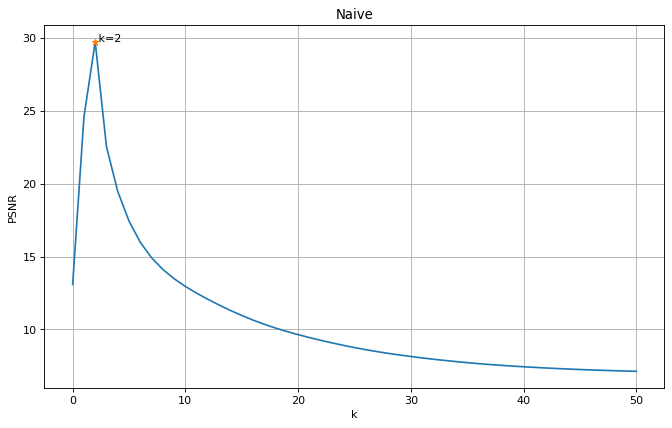
\includegraphics[width=10cm]{semiconvergenza/1/psnr_naive.png}
    \caption{PSNR al variare del numero delle iterazioni}
    \label{fig:semiconv_psnr_naive1}
\end{figure}
\begin{figure}[H]
    \centering
    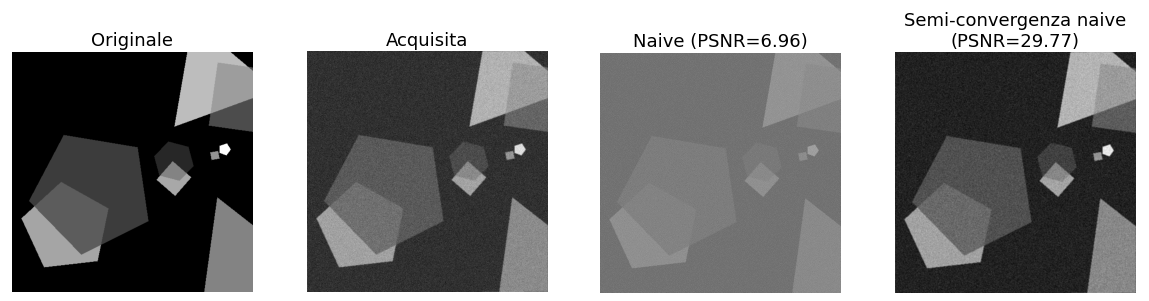
\includegraphics[width=8cm]{semiconvergenza/1/deblur_naive.png}
    \caption{Risultato ottenuto}
    \label{fig:semiconv_deblur_naive1}
\end{figure}
Come atteso, il risultato viene distorto molto rapidamente e non viene raggiunta convergenza nel punto ottimo.

\subsubsection{Regolarizzazione di Tikhonov}
\begin{figure}[H]
    \centering
    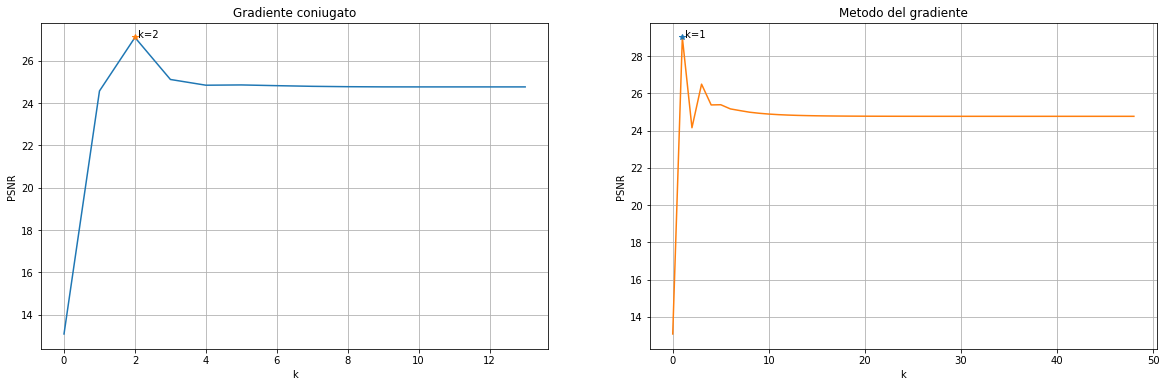
\includegraphics[width=15cm]{semiconvergenza/1/psnr_tikhonov.png}
    \caption{PSNR al variare del numero delle iterazioni}
    \label{fig:semiconv_psnr_tikhonov1}
\end{figure}
\begin{figure}[H]
    \centering
    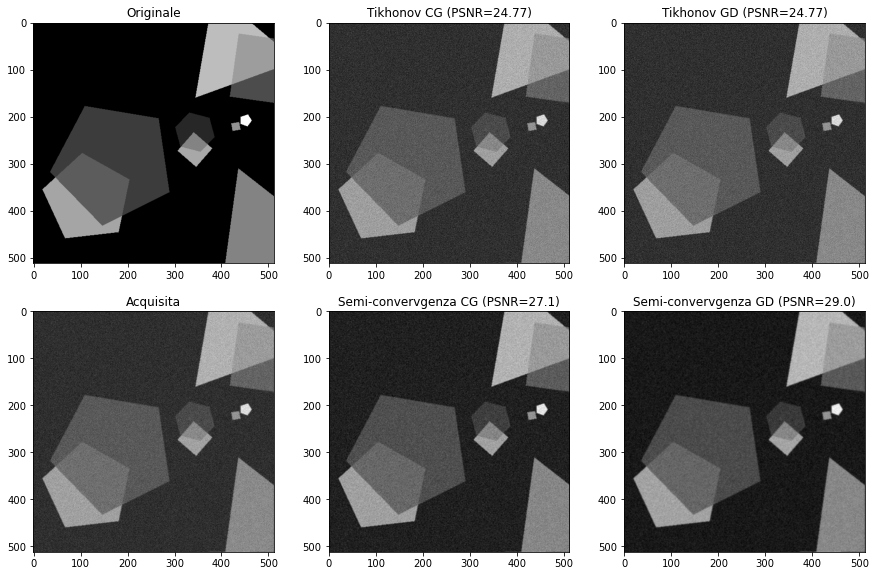
\includegraphics[width=10cm]{semiconvergenza/1/deblur_tikhonov.png}
    \caption{Risultato ottenuto}
    \label{fig:semiconv_deblur_tikhonov1}
\end{figure}
La regolarizzazione di Tikhonov viene introdotta per ridurre l'impatto del rumore sul risultato finale. 
Infatti si nota che, nonostante sia ancora presente il problema di semi-convergenza, dopo il punto di ottimo l'errore decresce di una quantità più contenuta rispetto al metodo naive fino ad assumere un comportamento asintotico.

\subsubsection{Regolarizzazione tramite variazione totale}
\begin{figure}[H]
    \centering
    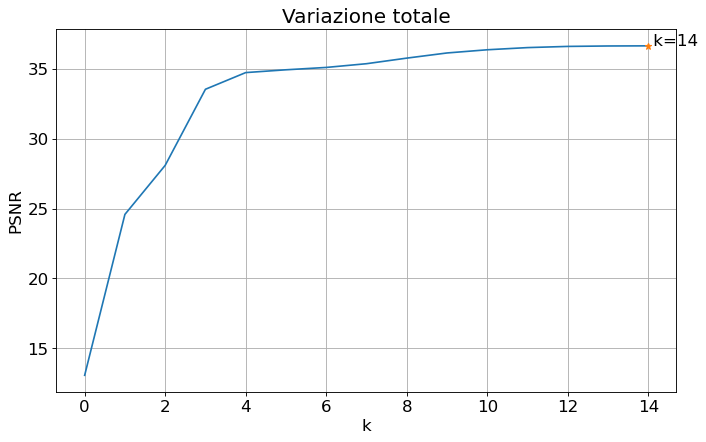
\includegraphics[width=10cm]{semiconvergenza/1/psnr_tv.png}
    \caption{PSNR al variare del numero delle iterazioni}
    \label{fig:semiconv_psnr_tv1}
\end{figure}
\begin{figure}[H]
    \centering
    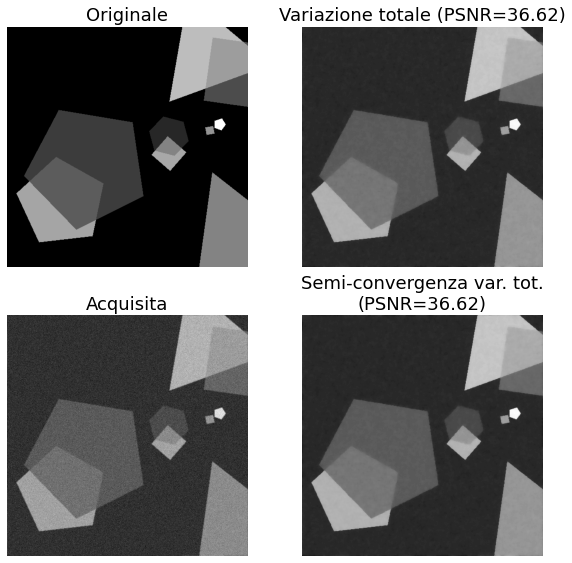
\includegraphics[width=8cm]{semiconvergenza/1/deblur_tv.png}
    \caption{Risultato ottenuto}
    \label{fig:semiconv_deblur_tv1}
\end{figure}
Regolarizzando tramite variazione totale invece, il problema di semi-convergenza è assente e il raggiungimento dell'ottimo avviene contemporaneamente al soddisfacimento delle condizioni di convergenza.

\subsubsection{Considerazioni finali}
Le prove precedenti sono state eseguite con kernel $5 \times 5$ con $\sigma=0.5$ e kernel $24 \times 24$ con $\sigma=3$, entrambi i casi con rumore con deviazione standard $]0, 0.05]$.\\
Nel caso generale, non è possibile risolvere il problema di semi-convergenza interrompendo l'esecuzione quando si rileva l'aumento dell'errore, 
infatti come si è visto in \autoref{fig:semiconv_psnr_tikhonov1} nel caso del metodo del gradiente, l'andamento del PSNR assume più punti di massimo locale.

\subsection{Analisi senza rumore}
Si eseguono ora gli stessi esperimenti su un'immagine a cui è stato applicato un blur senza aggiungere rumore.
\begin{figure}[H]
    \centering
    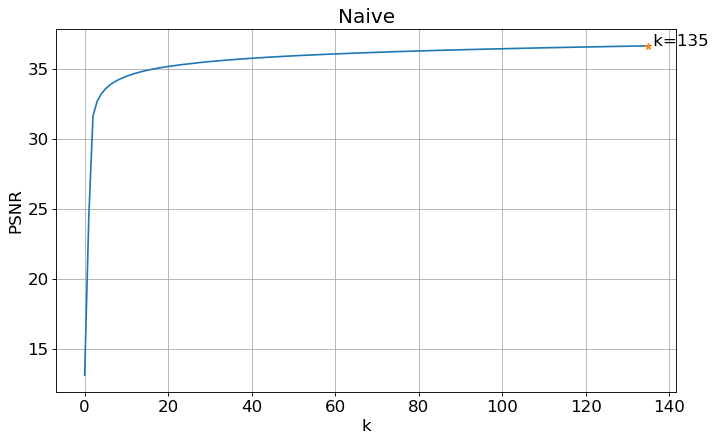
\includegraphics[width=8cm]{semiconvergenza/3/psnr_naive.png}
    \caption{PSNR al variare del numero delle iterazioni con il metodo naive}
    \label{fig:semiconv_psnr_naive3}
\end{figure}
\begin{figure}[H]
    \centering
    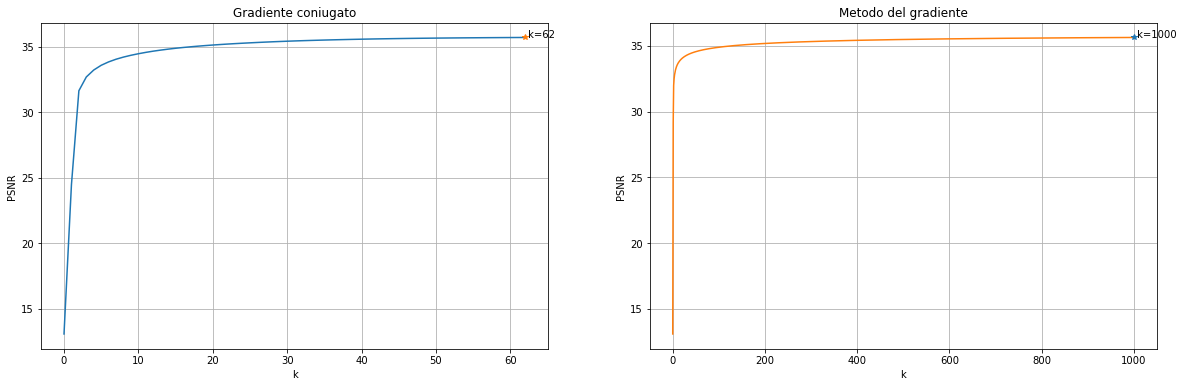
\includegraphics[width=15cm]{semiconvergenza/3/psnr_tikhonov.png}
    \caption{PSNR al variare del numero delle iterazioni con regolarizzazione di Tikhonov}
    \label{fig:semiconv_deblur_tikhonov3}
\end{figure}
\begin{figure}[H]
    \centering
    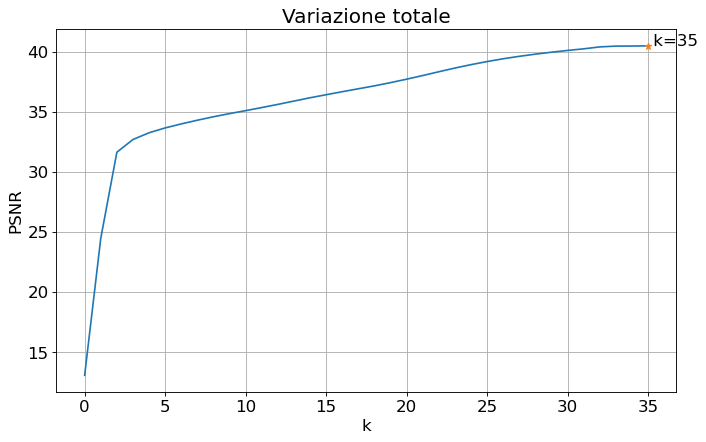
\includegraphics[width=8cm]{semiconvergenza/3/psnr_tv.png}
    \caption{PSNR al variare del numero delle iterazioni con regolarizzazione tramite variazione totale}
    \label{fig:semiconv_deblur_tv3}
\end{figure}
\begin{figure}[H]
    \centering
    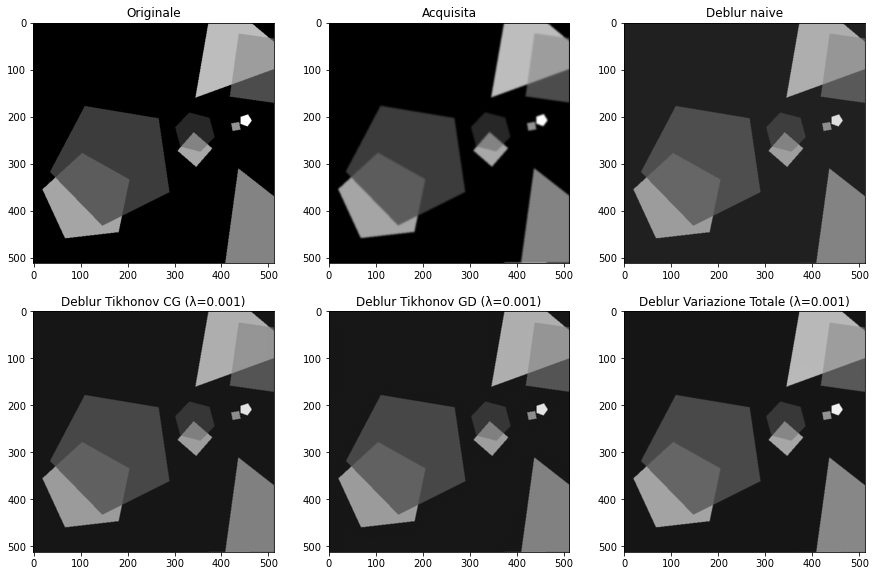
\includegraphics[width=10cm]{semiconvergenza/3/deblur_all.png}
    \caption{Risultato ottenuto}
    \label{fig:semiconv_deblur3}
\end{figure}
Come atteso tutti i metodi hanno raggiunto convergenza e ottimo contemporaneamente e il risultato, in assenza di rumore, si presenta molto simile indipendentemente dalla formulazione.

\section{Risultati su esecuzioni multiple}



% # Relazione

% 1. Riportare e commentare i risultati ottenuti nei punti 2. 3. (e 4.) su un immagine del set creato e su altre due immagini in bianco e nero  (fotografiche/mediche/astronomiche)
% 2. Riportare delle tabelle con le misure di PSNR e MSE ottenute al variare dei parametri (dimensione kernel, valore di sigma, la deviazione standard del rumore, il parametro di regolarizzazione). 
% 3. Calcolare sull’intero set di immagini medie e deviazione standard delle metriche per alcuni valori fissati dei parametri.  
% 4. Analizzare su 2 esecuzioni le proprietà dei metodi numerici utilizzati (gradiente coniugato e gradiente) in termini di numero di iterazioni, andamento dell’errore, della funzione obiettivo, norma del gradiente. 


\end{document}